\documentclass{article}
\usepackage[utf8]{inputenc}
\usepackage{amsmath}
\usepackage{graphicx}
\usepackage{float}
\usepackage{xcolor} 
\usepackage{mathtools}
\usepackage{leftidx}

\definecolor{white}{RGB}{255,255,255}

\title{\huge \color{white} Cosmology and Dark Matter}
\author{\color{white} \Large Aswin Suresh\\
        \color{white} \small 20b030011\\
        \color{white} \normalsize Mentor: Muskan Jain}
\date{\color{white} Summer 2021}

\usepackage{watermark}
\thiswatermark{\centering \put(-140,-768){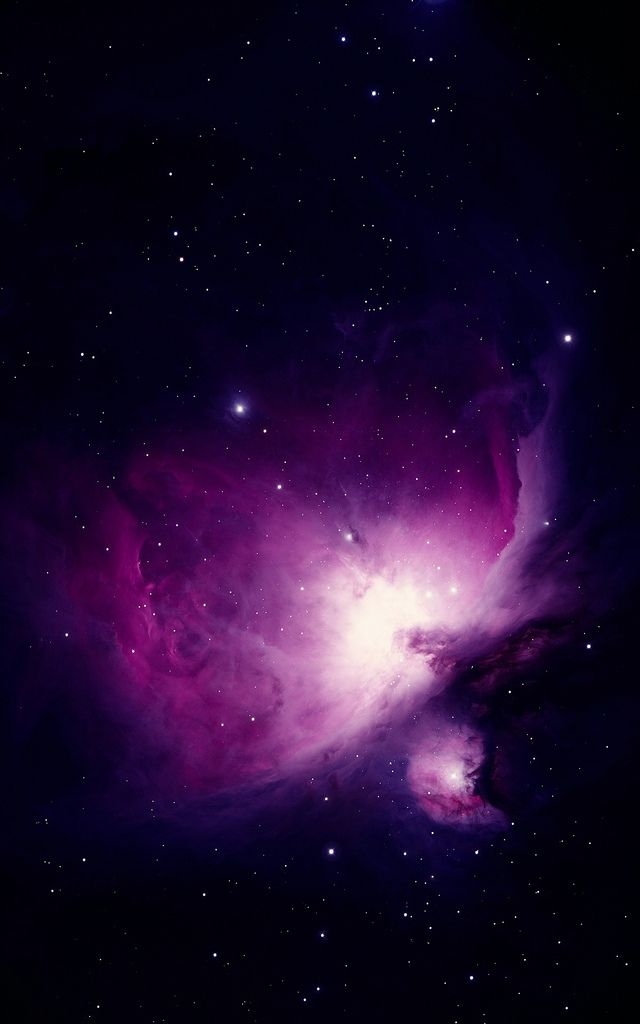
\includegraphics[scale=1.05]{background.jpg}}}

\begin{document}

\maketitle
\newpage
\tableofcontents
\newpage


\section{Friedmann Equation}
The Friedmann equation, describing the expansion of the universe, is one of the most important equations in cosmology. The equation can be derived completely from Newtonian theory, while General Relativity can be used to correct for outlying cases.

\subsection{Derivation}
Consider a particle of mass m at a distance r from a fixed point which may be assumed to be the centre of expansion, by virtue of the cosmological principle. The kinetic and potential energies of the particle will be given by:

\begin{center}
    $T = \frac{1}{2}m\dot{r}^2$ \\
\end{center}

\begin{center}
    $V = -\frac{GMm}{r} = -\frac{4\pi G \rho r^2 m}{3}$
\end{center}

Using Newton's laws, the total energy U \textbf{of the particle} given by the sum of potential and kinetic energies will be:

\begin{equation}
U = \frac{1}{2}m\dot{r}^2-\frac{4\pi}{3}G{\rho}r^2m
\end{equation}

The crucial step in the derivation is shifting the coordinates to a system called \textbf{comoving coordinates}, which can be expressed as $\vec{r}=a(t)\vec{x}$, where x is fixed for the particle under consideration, i.e $\dot{x}=0.$. Here a is known as the \textbf{scale factor of the Universe}, and gives information about how physical separation(r) changes with time.

\begin{figure}[H]
    \centering
    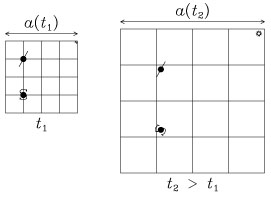
\includegraphics[width=0.5\textwidth]{figure1}
    \caption{Comoving coordinates}
    \label{fig:coord}
\end{figure}

\begin{center}
    $U = {\frac{1}{2}}{m{\dot{a}^2}{x^2}}-\frac{4\pi}{3}G{\rho}{a^2}{x^2}m$
\end{center}

Further simplification, after the above substitution, leads to the Friedmann equation:

\begin{equation} \label{eq:1}
(\frac{\dot{a}}{a})^2 = \frac{8{\pi}G}{3}\rho -\frac{kc^2}{a^2}
\end{equation}

The left hand side of the equation is independent of spatial coordinates, implying that $k = -\frac{2U}{m{c^2}{x^2}}$ must also be independent of x. Therefore $U \propto {x^2}$.The constant k, is related to the curvature of space and will be used extensively in further analysis. \\

NOTE: The expansion of the universe makes sense only at very large distance scales (such as at mega-parsec scale), as the universe is expected to appear uniform then. 

\subsection{Fluid and Acceleration equations}
Information about the mass density of the universe is necessary to obtain a solution of the Friedmann equation. This is given by a differential equation involving the pressure p, of material and is called the fluid equation. It can be obtained from the first law of thermodynamics: $dE+pdV = TdS $. I the comoving radius x is set to 1, then:

\begin{center}
    $E = mc^2 = \frac{4\pi}{3}a^3{\rho}c^2$ \\
\end{center}
    
\begin{center}    
    $\frac{dE}{dt} = 4{\pi}a^2{\rho}c^2\frac{da}{dt}+\frac{4\pi}{3}a^3c^2\frac{d\rho}{dt}$
\end{center}

Using $\frac{dV}{dt} = 4{\pi}a^2\frac{da}{dt}$ and assuming reversible adiabatic expansion (dS=0), the fluid equation comes out as:

\begin{equation} \label{eq:2}
    \dot{\rho}+3\frac{\dot{a}}{a}(\rho+\frac{p}{c^2})=0
\end{equation}

Although a pressure term appears in the above equation, it is important to note that in a homogeneous universe, no pressure gradients exist, implying that force does not aid in expansion of space. Pressure only contributes to work done.
\\
The acceleration equation can be obtained by differentiating equation \ref{eq:1} with respect to time and substituting $\dot{\rho}$ from \ref{eq:2}. This gives:

\begin{center}
    $\frac{\ddot{a}}{a}-(\frac{\dot{a}}{a})^2=-4{\pi}G(\rho+\frac{p}{c^2}+\frac{kc^2}{a^2}$
\end{center}

Substituting $\frac{\ddot{a}}{a}$ from equation \ref{eq:1} again, we obtain the \textbf{acceleration equation}:

\begin{equation}
    \frac{\ddot{a}}{a}=\frac{-4{\pi}G}{3}(\rho+\frac{3p}{c^2})
\end{equation}

Typically, the value of c is set to 1 in cosmology, making time and length, as well as mass and energy interchangeable. Hence the $c^2$ term in the Friedmann equation is often dropped, giving k the unit of $[time]^{-2}$.

\subsection{Interpretation of $k$}

The term $k$ which appears in the Friedmann equation is related to the curvature of space, in the purview of general relativity. Corresponding the different values of $k$, different goementries are possible for the universe; namely flat (corresponding to $k$=0), spherical (corresponding to $k>0$) and hyperbolic (corresponding to $k<0$).

\begin{itemize}
    \item Flat geometry: As is clear from the name, this would correspond to a two dimensional plane universe, where Euclidean geometry principles hold (the shortest distance between two point is a straight line and parallel lines are e fixed distance apart). This is usually called \textbf{flat universe}.
    \item Spherical geometry: This corresponds to a closed structure, with no boundary and fixed area, where Euclidean axioms do not hold. In fact it is one of the simplest non-Euclidean geometries known. The symmetry of the sphere preserves isotropy as well. This case is referred to as \textbf{closed universe}.
    \item Hyperbolic geometry: This represents a saddle type structure which, again, does not satisfy Euclidean norms and 'parallel lines' diverge from each other. This is referred to as \textbf{open universe}.
\end{itemize}

The open and flat would mean that the universe is infinite at any finite time. It could still continue expanding in the sense that distance between objects in it continue to increase. There is no way to confirm whether this is the case as we can only see a small part of the universe, restricted by the speed of light, known as the \textbf{observable universe}.

\begin{figure}[H]
    \centering
    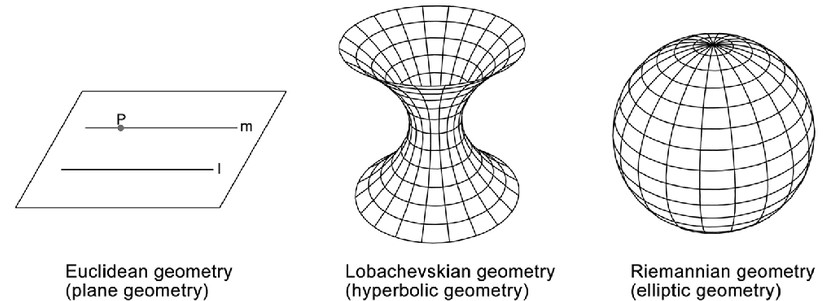
\includegraphics[width=\textwidth]{figure 4.jpg}
    \caption{These are the three postulated geometries of the universe corresponding to different values of $k$, as described above}
    \label{fig:matrad}
\end{figure}

\section{Cosmological Models}
\subsection{Hubble's constant and the scale factor}

The Hubble's constant can be expressed using the Friedmann equation. We know that the recession velocity $ \vec{v} = \frac{d\vec{r}}{dt} $. Since $ \vec{r}=a\vec{x} $ and $ \vec{x}$ is constant, we get $ \vec{v} = \frac{\dot{a}}{a}\vec{r} $. Hence using Hubble's law, we can say that $ H=\frac{\dot{a}}{a} $. Hence the term H can be substituted in Friedmann equation to obtain:

\begin{equation}
    H^2 = \frac{8{\pi}G}{3}\rho - \frac{k}{a^2}
\end{equation}

Furthermore, the relation between wavelength of observed light and the scale factor can be obtained using Hubble's law. The relative velocity between two nearby objects, such as galaxies is gievn by $dv = Hdr = \frac{\dot{a}}{a}r$. Since the objects are assumed to be nearby, we can say that $d\lambda = \lambda_{r}-\lambda_{e}$ (wavelength received - wavelength emitted). According to Doppler's law , $\frac{d\lambda}{\lambda_{e}} = \frac{dv}{c}$.Since the wavelength gets redshifted when emitting object moves farther away, ${d\lambda}$ is positive.

\begin{center}
\begin{math}
    \frac{d\lambda}{\lambda_{e}} = \frac{\dot{a}}{a}\frac{dr}{c} = \frac{\dot{a}}{a}dt = \frac{da}{a}
\end{math}
\end{center}


\begin{center}
    $\implies{\lambda \propto a}$
\end{center}

The increase in wavelength can also be thought of as wavelength getting "stretched" due to the expansion of space. The redshift, z, is defined as :

\begin{center}
    $1+z = \frac{\lambda_{r}}{\lambda_{e}} = \frac{a(t_r)}{a(t_e}$
\end{center}

\subsection{Solutions to Friedmann Equation}
In order to solve the Friedmann equation, we need information about the pressure and density of the universe, which will be described by an equation called equation of state. 

The universe is believed to consist of matter and radiation. Matter refers to non-relativistic material in cosmology while radiation includes all relativistic particles (typically photons and neutrinos). Matter has negligible pressure ($p = 0$) and radiation has a pressure given by $p = \frac{{\rho}c^2}{3}$.

The Friedmann equation has a crucial element of symmetry; the scale factor always appears as a fraction ${\dot{a}}{a}$, which means that it can be scaled according to our convenience. Hence we take the value of a at present time to be 1. The value of $k$ is assumed to be \textbf{zero} in this analysis. 

\begin{itemize}
    \item Case 1: Matter: \\
    Taking p to be 0 in the fluid equation gives the following:
    \begin{center}
    \begin{math}
         \dot{\rho} + 3\frac{\dot{a}}{a}{\rho} = 0 \implies \ln(\rho) = -3\ln{a} + const \implies \rho \propto \frac{1}{a^3}
    \end{math}
    \end{center}
    In cosmology, the present value of parameters is usually represented by a subscript. Hence, 
    ${\rho}=\frac{{\rho}_0}{a^3}$. Substituting this in the Friedmann equation gives ${\dot{a}^2} = \frac{8{\pi}G{\rho_{0}}}{3}\frac{1}{a}$.
    This equation can further be solved, from which we obtain a power law solution $a(t)=(\frac{t}{t_0})^{\frac{2}{3}}$ and $H=\frac{2}{3t}$.
    \item Case 2: Radiation: \\
    The presence of radiation pressure $p = \frac{{\rho}c^2}{3}$ changes the fluid equation from the matter dominated case and leads to the following:
    \begin{center}
    \begin{math}
         \dot{\rho} + 4\frac{\dot{a}}{a}{\rho}=0 \implies \rho \propto \frac{1}{a^4}
    \end{math}
    \end{center}
    This is again substituted in the Friedmann equation and another power law solution is obtained. a(t) = $(\frac{t}{t_0})^{\frac{1}{2}}$
    \item Case 3: Mixtures: \\
    When both matter and radiation are present, which is what is expected in our universe, the total density $\rho$ is given as sum of densities of matter and radiation components. Obtaining $\rho$ as a function of time is not simple when $\rho_{mat}$ and $\rho_{rad}$ have approximately equal contributions to total density, but can be analysed when one dominates over the other. In both cases we obtain that matter domination is more stable as matter density falls slower compared to radiation density. Hence the universe would eventually end up being dominated by matter in its later stages.
\end{itemize}

\begin{figure}[H]
    \centering
    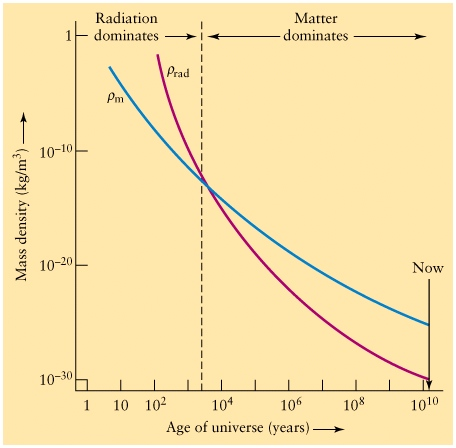
\includegraphics[width=0.6\textwidth]{figure 2.jpg}
    \caption{This plot shows how the density contribution from matter and radiation changes over time. It can be seen that the Universe starts out being dominated by radiation, which then shifts to matter, due to reasons cited earlier.}
    \label{fig:geometry}
\end{figure}

The way the universe evolves can change depending on the value of $k$ as well. Since the expansion of the universe is governed by the scale factor a and rate of expansion by $\dot{a}$, the Hubble factor, being a ratio of the two, is a good measure of expansion. The universe will stop expanding when H=0. 

Hence it is evident that H cannot be zero when k is negative or 0. In fact when k is negative the density factor becomes negligible compared to the $k$ term, leading to $a \propto t$. This is known as \textbf{free expansion} as the velocity of expansion is 0.

When $k>0$, H must become 0 at one point in time since the $k$ term will become large enough to cancel out the density term. Hence re-collapse of the universe will happen in closed geometries.

\subsection{Observational Parameters}
Since the Friedmann equation isn't constant in time, certain factors such as present expansion rate, present density etc. need to be fixed by observation. 

The first parameter is the Hubble constant $H_0$, which is also the expansion rate of the universe. It can be calculated using Hubble's law if velocity and distance of astronomical objects are known. Velocities are obtained from redshift measurements, but this measured velocity also has a component of velocity corresponding to the relative motion of objects (called \textbf{peculiar velocity}), in addition to the universe's rate. This issue is overcome by measuring velocities if object which are very far away, since cosmological principle demands that the peculiar velocity be independent of the scale of the universe. Distance measurement using standard candles, such as Cepheid variables or supernovae enables us to calculate $H_0$. State of the art measurements have calculated it to a good accuracy, giving $H_0=100h$ $kms^{-1} Mpc^{-1}$, where $h=0.72\pm0.08$ is an uncertainty factor. \\

The second parameter is the density parameter. From the equation $H^2 = \frac{8{\pi}G}{3}\rho - \frac{k}{a^2}$, we can see that for a given H, there exists a corresponding value of $\rho$ such that $k$ goes to zero. This density is knows as the critical density:

\begin{equation}
    \rho_{c}(t) = \frac{3H^2}{8{\pi}G}
\end{equation}

$\rho_{c}$ changes with time due to its dependence on H. Plugging in the present value of the Hubble's constant gives the value of critical density to be $1.88h^2$ x $10^{-26}$ $kgm^{-3}$, which is a very small value of density compared to objects in everyday life. However, when it is expressed in units of $[Solar Mass][Mpc]^{-3}$, its value is of the order of $10^11$. Eventhough the universe may not be flat, the critical density sets a good scale for comparison. Hence the \textbf{density parameter}, $\Omega$ is defined as 

\begin{center}
    $\Omega(t) = \frac{\rho}{\rho_c}$
\end{center}

$\rho$ can be substituted back in the Friedmann equation as $\Omega\rho_c$:

\begin{center}
\begin{math}
  H^2 = \frac{8{\pi}G}{3}{\rho_c}\Omega - \frac{k}{a^2} = H^2\Omega - \frac{k}{a^2}
\end{math}
\end{center} 

\begin{center}
    $\implies \Omega = 1 + \frac{k}{a^2H^2}$
\end{center}

Hence we can see that $k=0$ when $\Omega = 1$

A density parameter corresponding to $k$ can also be defined as $\Omega_k = -\frac{k}{a^2H^2}$, which implies that $\Omega+\Omega_k=1$ \\

The final observation parameter, which is dependent on the above two, is called the \textbf{deceleration parameter}. It can be obtained as follows: 

\begin{center}
\begin{math}
    a(t) = a(t_0) + \dot{a}(t_0)[t-t_0] + \frac{1}{2}\ddot{a}(t_0)[t-t_0]^{2}...
\end{math}
\end{center}

\begin{center}
\begin{math}
   \implies \frac{a(t)}{a(t_0)} = 1+ H_0[t-t_0] - \frac{q_0}{2}H_0^2[t-t_0]^2 + ...
\end{math}
\end{center}

This defines the deceleration parameter $q_0$ as $q_0 = \frac{\ddot{a}(t_0)}{a(t_0}\frac{1}{H_0^2}$. Since $q_0 \propto \ddot{a}(t_0)$, higher its value, faster will be the deceleration. In case of matter dominated universe, $q_0 = \frac{\Omega_0}{2}$. Since $q_0$ is easier to measure, we can obtain values of other parameters from it. Recent observation have shown that $q_0<0$, which means that our universe is accelerating, which is not possible in the models defined earlier. To correct this another parameter was introduced in the Friedmann equation called the \textbf{cosmological constant}.

\section{Cosmological Constant}
\subsection{Introduction}
While formulating the theory of General relativity, an extra parameter was introduced to the equations in order to keep the universe static. Eventhough this idea is incorrect the \textbf{cosmological constant, $\Lambda$}, is an important part of cosmology and the Friedmann equation is modified as:

\begin{equation}
    H^2 = \frac{8\pi{G}}{3}\rho - \frac{k}{a^2} + \frac{\Lambda}{3}
\end{equation}

The original idea was to cancel out the effects of the first two terms, which is obviously incorrect since a static universe is not stable to small perturbations. From the above equation a new acceleration equation can be derived, from which we obtain that the cosmological constant makes a positive contribution to acceleration of the universe. Similar to a density parameter corresponding to $k$, a density parameter corresponding to $\Lambda$ can be defined and calculated as:

\begin{center}
    $\Omega_{\Lambda} = \frac{\Lambda}{3H^2}$
\end{center}

Incorporating this into the density equation gives:

\begin{center}
    $\Omega+\Omega_{\Lambda}-1 = \frac{k}{a^2H^2}$
\end{center}

This implies that for a flat universe ($k=0$) \textbf{$\Omega+\Omega_{\Lambda}=1$}. The density term arising from the cosmological constant is typically not considered ti be a part of matter density. Depending on the value of k the sum of $\Omega$ and $\Omega_{\Lambda}$ vary. They are between 0 and 1 for an open universe, 1 for flat and grater than 1 for closed universe.

\subsection{New cosmological models}
If we define a new quantity \textbf{$\rho_{\Lambda}$} = $\frac{\Lambda}{8\pi{G}}$, then substituting this back in the modified Friedmann equation will combine the two density factors:

\begin{center}
    $H^2 = \frac{8\pi{G}}{3}(\rho+\rho_{\Lambda}) - \frac{k}{a^2}$
\end{center}

This can be interpreted as contribution from a fluid of energy density $\rho_{\Lambda}$ and density parameter $\Omega_{\Lambda} = \frac{\rho_{\Lambda}}{\rho_c}$. If the density value is substituted in the fluid equation in order to obtain the pressure from the cosmological constant, we obtain $p_{\Lambda} = -\rho_{\Lambda}c^2$. The negative value of pressure implies that the expansion of the universe does work on this hypothetical fluid, enabling it's energy density to remain constant. 

$\Lambda$ can be interpreted physically as the energy density corresponding to free space, similar to the existence of zero-point energy in quantum physics. This also gives rise to the cosmological constant problem, due to present theoretical models predicting this energy to be far greater than observed.

It can be observed that the inclusion of the cosmological constant no longer imposes many restrictions on the state and structure of the universe depending on $k$. Theoretically, many models of the universe having varying initial conditions are possible, although many of those are rendered moot though observations.

As discussed in the previous section, we can express the deceleration parameter including the cosmological constant as 

\begin{center}
    $q_0 = \frac{\Omega_0}{2} - \Omega_{\Lambda}$
\end{center}

From this equation it can be inferred that $q_0<0$ when $\Omega_{\Lambda} > \frac{\Omega}{2}$. If a flat geometry is assumed then this relation reduces to $\Omega_{\Lambda} >\frac{3\Omega_0}{2}-1 $ and the universe will accelerate if $\Omega_{\Lambda} > \frac{1}{3}$.


These possibilities are usually plotted on a figure with $\Omega_0$ and $\Omega_{\Lambda}$ as axes:

\begin{figure}[H]
    \centering
    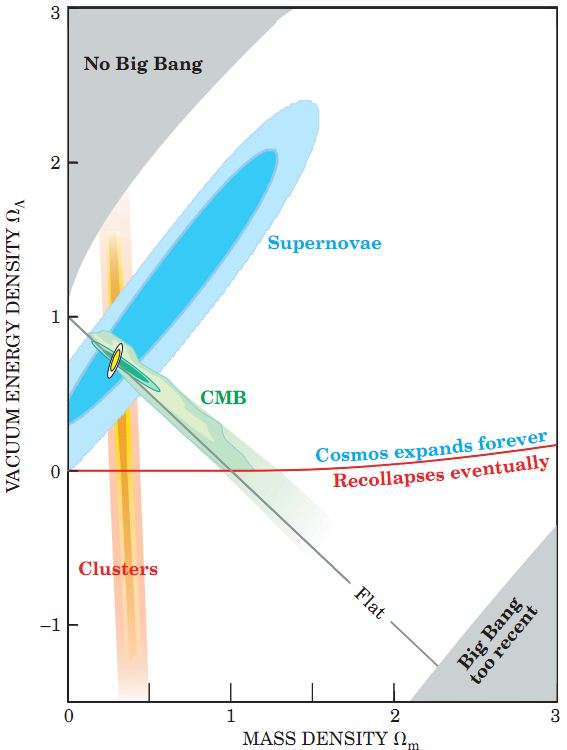
\includegraphics[width=\textwidth]{figure 5.jpg}
    \caption{Values of $\Omega_{\Lambda}$ are plotted against $\Omega_m$ (normalised mass density), along with observations of three phenomena: high red-shift supernovae, CMB and galaxy clusters. The three are shown to converge nicely at $\Omega_m = 0.3$ and $\Omega_{\Lambda} = 0.7$. It can be seen that $\Omega_m+\Omega_{\Lambda} =1$, implying flat geometry. It turns out that a good estimate of the universe's age is also obtained corresponding to these values of density perimeters}
    \label{fig:density}
\end{figure}


%REMEMBER TO CHANGE THE ORDER HERE

\subsection{Age of the Universe}
The cosmological models obtained from the Friedmann equation and the cosmological constant can be used to estimate the age of the universe. The obtain a crude estimate, consider the Hubble parameter. Being the rate of expansion of the universe, it can also be written in the form $r = v H_0^{-1}$, implying that the inverse of it's value is a good timescale to compare the universe age to. Given that the presnt value of the Hubble's constant is estimated to be $H_0 = 100h$ $km s^{-1} Mpc^{-1}$, $H_0^{-1}$ comes out to be $9.77h^{-1}$ x $10^9$ years. This quantity is also called \textbf{Hubble time}. Observation of globular clusters and chemical and thermonuclear activities in stars, as well as obtaining an estimate of the Earth's age, puts the estimated age of the universe between 10-15 billion years. 

A more rigorous calculation can be done by assuming the universe to be matter dominated. This claim is sensible since the a matter dominated universe is more stable, hence this phase can be expected to be present since a considerable time. Hence,

\begin{center}
    $a(t) = (\frac{t}{t_0})^{\frac{2}{3}}$
\end{center}

\begin{center}
    $\implies H = \frac{\dot{a}}{a} = \frac{2}{3t}$
\end{center}

This means that the present time, $t_0 = \frac{2}{3}H_0^{-1}$, which predicts the age as 9.3 billion years, which is incorrect from observations. This value falls further if the universe is assumed to be closed. If the universe is considered open instead and $\Omega_{0}<1$, then the number increases. This is reasonable, since with less matter the amount of gravitational attraction pulling matter inwards would be less and hence it would take the universe a longer time to slow down the expansion rate to the present value. 

Present observations comply nicely with a model in which the universe is flat and density is low, while having a positive cosmological constant. These parameters can be set such that the age exceeds Hubble time:

\begin{equation}
    H_0t_0 = \frac{2}{3}\frac{1}{\sqrt{1-\Omega_0}}ln[\frac{1+\sqrt{1-\Omega_0}}{\sqrt{\Omega_0}}] = \frac{2}{3}\frac{1}{\sqrt{1-\Omega_0}}sinh^{-1}[\sqrt\frac{1-\Omega_0}{\Omega_0}]
\end{equation}

It can be obtained that $t_0 = H_0^{-1}$ when $\Omega_0 = 0.26$. Presently it is estimated that the age of the universe is 14 billion years with $\Omega_0 \approx 0.3$. This is in good agreement with experimental values.

\begin{figure}[H]
    \centering
    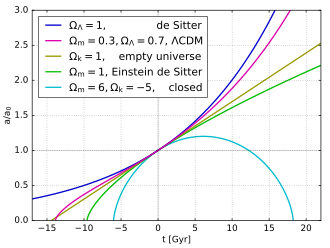
\includegraphics[width=\textwidth]{figure 3.png}
    \caption{Plots which can be used to determine the present age of the universe corresponding to different values of the density parameters. The inclusion of dark matter does alter calculations from those presented in this section.}
    \label{fig:age}
\end{figure}

\section{Dark Matter and CMB}
\subsection{Proof of existence of dark matter}

Similar to how the Hubble constant sets a scale to compare the age of the universe to, the critical density parameter does so for the actual density of the universe. Since information about stellar mass and distance is already available, it is possible to attempt to calculate the age of the universe using this. Hence this was done and it was obtained that $\Omega_{stars} = \frac{\rho_{stars}}{\rho_c}\rightarrow 0.01$.
\\
This means that the visible baryonic matter content of the universe is not enough to ensure that the universe's density approaches the critical value. Hence the theory of nucleosysnthesis was proposed, and demands that conventional material cannot contribute an entire critical density and in fact placed a limit on the baryonic density:

\begin{center}
    $0.021 \leq {\Omega_B}h^2 \leq 0.025$
\end{center}

Since the lower limit predicted is higher than observed, there must be more baryonic matter than observed in stars. This is true and had been confirmed by observation of galaxy rotation curves. Since galaxies have differential rotation curves it is expected that the circumferential velocity of stars evolves as $\frac{1}{\sqrt{R}}$, implying that it must reduce as distance from the centre of the galaxy increases. However on it was observed that the velocity remained approximately constant at larger radii, posing an evident contradiction. Since the circumferential velocity is also a function of mass enclosed between 0 to R it can be reasoned that the amount of mass increases along with radius, rather than stay constant as expected initially. This extra mass is what we call \textbf{dark matter}. 
\\
The calculated density of the dark matter halo comes out to be $\Omega_{halo} \approx 0.1$. It is expected that the dark matter is in the form of a spherical halo due to lack of any mechanism of collapse, owing to its extremely weak interaction.

\begin{figure}[H]
    \centering
    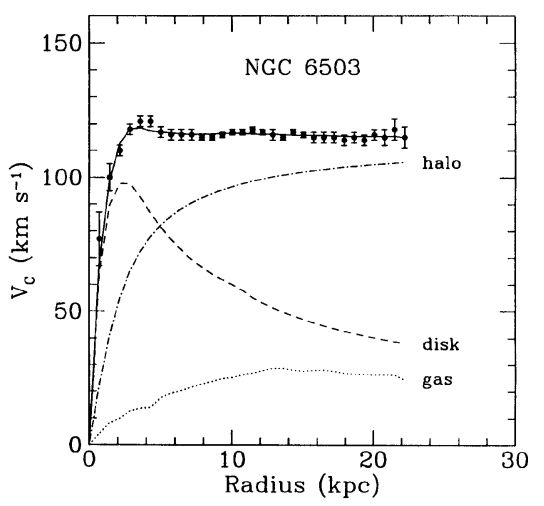
\includegraphics[width=0.8\textwidth]{figure6.jpg}
    \caption{The galaxy rotation curve of the galaxy NGC 6503 is shown here. Plots of the contributions from the three components, namely halo, disk and gas are also shown. The net result is a sum of the three.}
    \label{fig:curvesrotation}
\end{figure}

\subsection{Large Scale Structure}
Observations of galaxy clusters has lead to the conclusion that the density of hot gas component is 5 to 10 times higher than the density contribution form stars, which is also in agreement with their observed abundances.
\\
Observations of this hot gas have also enabled estimation of amount of dark matter present since the gravitational attraction from the cluster and surrounding gas is not enough to counter the thermal pressure from the gas. Hence the amount of dark matter can be estimated as:

\begin{center}
   $\frac{\Omega_B}{\Omega_0} \approx 0.065 h^{-\frac{3}{2}}$
\end{center}

Applying the nucleosysnthesis constraint gives the density parameter value as 0.4, suggesting the dark matter contribution is significantly higher than baryonic contribution. Further observation and analysis of the large scale structure of the universe and it anisotropies have cemented the idea that non-baryonic matter such as dark matter does indeed exist.

Finally measurement of the geometry of the universe was also carried out by some satellites (such as Planck) and have lead to the conclusion that \textbf{the universe is close to spatially flat} geometry, with $\Omega_0 \approx 0.3$ and $\Omega_{\Lambda} \approx 0.7$. This is also backed up by the theory if cosmological inflation.

\subsection{Nature of dark matter}
At present there is no clear idea of what constitutes dark matter, but there are some theoretical predictions from particle physics. One favourable dark matter candidate is the neutrino, assumed mass-less in cosmology but almost certainly has mass according to experiments being done currently. Neutrinos are extremely weakly interacting particles. There are three types of neutrinos: electron neutrino, muon neutrino and tau neutrino and present experiments place the latter two on a higher probability of being a dark matter candidate.
\\
Since the mass of neutrinos haven't been clearly determined, light and heavy neutrinos could lead to different kinds of dark matter namely hot dark matter (relativistic) and cold dark matter respectively.

Other particles proposed as dark matter candidates are the Light Supersymmetric Particle (LSP) and Weakly Interacting Massive Particles (WIMP).

\subsection{Cosmic Microwave Background}

\begin{figure}[H]
    \centering
    \includegraphics[width=0.8\textwidth]{figure 7.png}
    \caption{The cosmic microwave background}
    \label{fig:CMB}
\end{figure}

The CMB behaves similar to a black body with a temperature of $2.725 \pm 0.001 k$. When the energy corresponding to it is converted and written in terms of the critical density it come ou to be $\Omega_{rad} = 2.47$ x $10^{-5} h^{-2}$, which implies that it contributes to a small fraction of the universe's density.
\\
Stefan's law states that
\begin{center}
    $\epsilon_{rad} = \rho_{rad}c^2 = \frac{{\pi}^2{k_B}^4}{15{\hbar}^3c^3}T^4$
\end{center}

Since $\rho_{rad}$ evolves as $\frac{1}{a^4}$, it turns out that $T \propto \frac{1}{a}$, which means that the temperature of the universe must have been arbitrarily large in its beginning stages. Another element associated with this concept is the conservation of particle number. Given that the interactions between baryons and photons are negligible, their number density must be preserved as the universe expands. Hence 

\begin{center}
    $n_{\gamma} = \frac{\epsilon_{rad}}{E_{rad}} = 3.7$ x $10^8 m^{-3}$
\end{center}

\begin{center}
    $n_{B} = \frac{\epsilon_{B}}{E_{B}} = 0.25 m^{-3}$ 
\end{center}

The smaller number of baryons is due to the fact that their mass-energy is much higher, despite having higher energy density than photons.
\\
The origin of the CMB can be understood by considering the interaction between atoms and photons in the early universe. When the temperature was much higher, say $3$x$10^6 K$, the average energy of photons is enough to ionize the hydrogen atom from its ground state,which means that atoms could not be formed. Hence the early universe was a sea of electrons, protons and photons.
When the universe eventually cooled down, the average energy of photons fell and were not enough to ionize hydrogen completely. This event is called \textbf{decoupling}, wherein the universe suddenly changed from being completely opaque to transparent.
\\
A crude estimate can be obtained by comparing the average energy of photons $(3k_{B}T)$ to the ionization energy of hydrogen which is 13.6 eV. Dividing these quantities gives the temperature as 50000K. 
This is actually incorrect, even for an estimate. The reason is that ionization of hydrogen will still continue when the average energy if photons is below 13.6 eV due to the presence of high energy photons in the tail of the Boltzmann distribution. Taking that into account gives a better estimate:

\begin{center}
    $T_{dec} = 7400 K$
\end{center}

There is yet another phenomena which needs to be taken into account, which is \textbf{recombination}.Recombination refers to the time period when the protons and electrons first combined to form atoms. Since this process is not instantaneous it does not coincide with decoupling. Since decoupling cannot happen before recombination happens, this makes the temperature obtain earlier higher than the actual value. This new value can be obtained by using the Saha equation:

\begin{equation}
    \frac{1-X}{X} \approx 3.8\frac{n_B}{n_{\gamma}}(\frac{k_{B}T}{m_{e}c^2})^{\frac{3}{2}}e^{\frac{E_0}{k_{B}T}}
\end{equation}

where X is the protons to baryons, indicating the amount of ionization.This implies that the ionization will be large is the RHS of the equation is small. Recombination is defined to correspond to $X = 0.1$, i.e the process is 90 percent complete. Using this to solve the equation gives the temperature of the universe at decoupling to be \textbf{3600 K}.
\\
The fact that the CMB is a black body radiation is well explained by this model as the photons and baryons were in thermal equilibrium before decoupling. Since then the photons would travel without interruption and reach us from the surface of last scattering.

\section{Early Universe}
\subsection{Introduction}
Similar to how the energy density of radiation was calculated before, it it possible to do the same for neutrinos, although it is not completely backed by experiments and observations. Theoretical models predict

\begin{center}
    $\Omega_{\nu} = 0.68\Omega_{rad} = 1.65$ x $10^{-5}h^{-2}$
\end{center}

This value is quite similar to that of $\Omega_{rad}$ and the sum of these densities gives the total density contribution from relativistic particles, $\Omega_{rel} = 4.15$ x $h^{-2}$.
The ratio of the density of relativistic and non-relativistic matter can also be obtained, after taking into account their varying dependence on $a$.

\begin{equation}
    \frac{\Omega_{rel}}{\Omega_{mat}} = \frac{4.15 \times 10^{-5}}{\Omega_{0}h^2}\frac{1}{a}
\end{equation}

So depending on the value of a, after normalising it's present value to 1 there will be a point where the matter and radiation densities become equal. This is called \textbf{matter-radiation equality} and it occurs when $a = a_{eq} = \frac{1}{24000\Omega_{0}h^2}$

Hence the previously derived equation of matter and radiation domination can be applied to the two regimes appropriately, assuming k=0 and $\Lambda = 0$, which are reasonable assumptions to make.
Since $a \propto t^{\frac{2}{3}} \implies T \propto t^{\frac{-2}{3}}$,, therefore

\begin{center}
    $\frac{T}{2.725 K} = (\frac{4 \times 10^7 sec}{t})^{\frac{2}{3}}$
\end{center}
 for $T<T_{eq} = \frac{2.725 K}{a_{eq}} = 66000 \Omega_{0}h^2K$. Calculating the time of matter-radiation equality from here gives the value as $t_{eq} = 1.0$ x $10^11\Omega_{0}^{-\frac{3}{2}}$. This can also be used to calculate the time of decoupling $t_{dec} \approx 10^13 = 350000 years$. This also tells that decoupling occurred in matter dominated epoch.
\\
At temperatures higher than ${t_{eq}}$, 

\begin{center}
    $\frac{T}{T_{eq}} = (\frac{t_{eq}}{t})^{\frac{1}{2}}$
\end{center}

and using Friedmann equation $H^2 = \frac{8{\pi}G}{3}$x$1.68$x${\frac{{\alpha}T^4}{c^2}}$ gives the final equation as

\begin{equation}
    (\frac{1 sec}{t})^{\frac{1}{2}} \approx \frac{T}{1.3 \times 10^10 K} = \frac{{k_B}T}{1.1 MeV}
\end{equation}

From this it can be concluded that the temperature of the universe was $1.3$x$10^10$ K when it was 1 second old and average energy of particles was 1.1 MeV. Hence at times before this, the particle energies become comparable to the binding energy of nuclei and hence photons would break the nucleus apart into protons and neutrons. Hence before the formation of nuclei, photons and electrons, it universe existed as a sea of protons, neutrons, electrons and photons. 
\\
At times much before this, till about $10^{-12}$ seconds, the energy of photons becomes so high that the protons ans neutrons themselves disintegrate into quarks. The epoch where quarks condense and form protons and neutrons is called the \textbf{quark-hadron phase transition}. Hadrons are the bound states of quarks. Experimental and observational evidence for this theory is yet to be obtained.
The highest energy produced by particle accelerators presently reached around 100 GeV, corresponding to a temperature of $10^15 K$. Nothing is known about the state of affairs before $10^{-10}$ seconds.

\subsection{Nucleosynthesis}
Study if stars and nebulae have enabled scientists to study about the elements produced by them by means of thermonuclear fusion. However it is not possible to produce light elements such as hydrogen and deuterium, which are assumed to be present in stars for further fusion. The theory if nucleosynthesis explains how the lighter elements are formed in the very early stages of the universe.
\\
In nucleosynthesis three facts are important: (i) Protons being lighter than neutrons, (ii) instability of free neutrons and they decay half life (610 seconds) and (iii) stability if neutrons in bound form, i.e. in nuclei. Starting the analysis from a point when nuclei do not exist, but protons and neutrons are non-relativistic, the distribution of number densities can be given by a Boltzmann distribution and a ratio can be obtained:

\begin{equation}
    \frac{N_n}{N_p} = (\frac{m_n}{m_p})^{\frac{3}{2}}e^[{-\frac{(m_n-m_p)c^2}{k_{B}T}]}
\end{equation}

Here the factor of mass ratio can be approximated to 1 and when $k_{B}T >> (m_n-m_p)c^2$ the exponential term also comes out to be one,implying that the number of protons and neutrons is approximately equal at high temperatures,such as the ones prevailing in the early universe.
The following reactions take place:

\begin{center}
    $n + \nu_{e} \xleftrightarrow p + e^{-}$
\end{center}

\begin{center}
    $n + e^{+} \xleftrightarrow p + {\bar{\nu}_{e}}$
\end{center}

where the electron neutrino and its anti particle are represented by $\nu_{e}$ and ${\bar{\nu}_{e}}$ respectively. The rate of interaction also dictates the thermal equilibrium condition and calculations predict that the reactions procced at a fast pace until $k_{B}T \approx 0.8$ MeV. At the end of the interaction period, the number densities remain approximately fixed as $\frac{N_n}{N_p} = \frac{1}{5}$.

This is followed by another set of reactions: 

\begin{center}
    $p + n \rightarrow D$
\end{center}

\begin{center}
    $D + p \rightarrow ^{3}He$
\end{center}

\begin{center}
    $D + D \rightarrow ^{4}He$
\end{center}

and these continue till the energy reaches about 0.06 MeV, which is obtained similar to the high energy photon decoupling calculation. Eventhough the age of the universe by this point is comparable to the half-life of the neutron, they manage to stay stable, which is very good for further processes taking place. The neutron proton ratio falls to $\frac{1}{7.3}$ at this stage.

\begin{figure}[H]
    \centering
    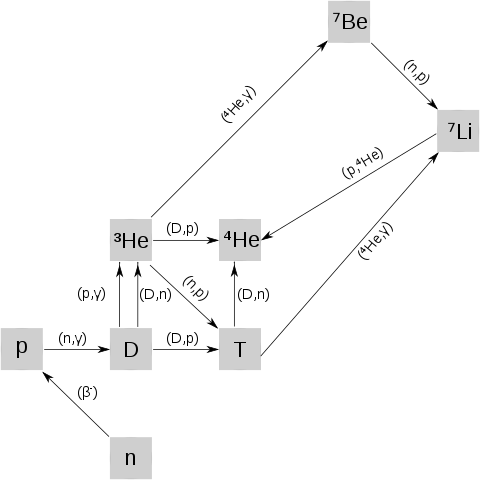
\includegraphics[width=0.8\textwidth]{figure 8.png}
    \caption{The reactions in nucleosynthesis}
    \label{fig:nsyn}
\end{figure}

The big bang theory predicted the existence of 3 kinds of neutrinos, in order for the equations to be derived and this was confirmed experimentally by the LEP experiment at CERN. The abundances of the other elements such as Hydrogen and Helium predicted from the theory also match nicely with observational evidence.

\begin{figure}[H]
    \centering
    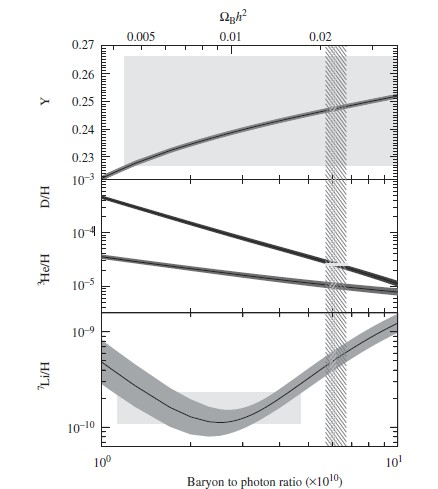
\includegraphics[width=0.8\textwidth]{figure 8.jpg}
    \caption{This plot shows the predicted abundances of light nuclei, on a scale of $\Omega_{B}h^2$ as well as baryon to photon ratio for Lithium-7, Helium-3 and Deuterium}
    \label{fig:abundance}
\end{figure}

\section{Inflationary Cosmology}
\subsection{Problems with the Big Bang model}
 There are three problems with the hot big bang model.
 \subsubsection{Flatness}
 Observations have concluded that total density $\Omega_{tot} = \Omega_0 + \Omega_{\Lambda}$ lies in the range 0.5 to 1.5, which makes the universe close to spatially flat. From the Friedmann equation we obtain that $|{\Omega_{tot}(t)-1}| \propto (a^2H^2)^{-1}$. From cosmological models, we know that $a^2H^2$ varies as $t^{-1}$ for radiation domination and as $t^{-\frac{2}{3}}$ for radiation domination implying that the difference between $\Omega_{tot}$ and 1 increase with time and the universe looses its flatness, but since the curvature contribution comes from $\frac{k}{a^2}$, it must be extremely small to begin with in order to not dominate the radiation and matter densities which go as $\frac{1}{a^3}$ and $\frac{1}{a^4}$ respectively. This poses an apparent dilemma since applying this to the models of nucleosynthesis, which is quite well established, given a very very small margin of the density parameter around 1.
 \subsubsection{Horizon Problem}
 This is one of the most important problems. It is a based on our observation of the cosmic microwave background. Since the observed radiation is very close to uniformity, it can be said that the different parts of the sky achieved thermal equilibrium. However since light from one part of the sky has just reached us in Earth, it is not possible for it to travel and interact with the opposite side of sky, which poses a contradiction to the claim of thermal equilibrium. The anisotropies of the CMB are also not explained properly.
 \subsubsection{ Particle abundances}
 The domination of radiation in the early stages of the universe is not completely compatible with the modern theories of unification and the big bang as well due to the absence of magnetic monopoles, which were predicted to be highly abundant in the very early stages of the universe but no evidence of their existence is known. Other such particles are also predicted but found to be incompatible with current models.
 
 \subsection{Inflation}
 The solution to these problems comes from inflation. It can be taken to be an epoch where the scale factor is accelerating, i.e. $\ddot{a(t)}>0$. 
 Hence from the acceleration equation 
 
 \begin{center}
     $\frac{\ddot{a}}{a} = -\frac{4{\pi}G}{3}(\rho + \frac{3p}{c^2}$
 \end{center}

we can see that$p<-\frac{{\rho}c^2}{3}$ for the scale factor to accelerate with time. This can be modeled as the cosmological constant acting as a  fluid with pressure $-{\rho}c^2$. From the Friedmann equation modified with the cosmological constant, taking the first two terms to be negligible compared to $\Lambda$. Hence 

\begin{equation}
    H^2 = \frac{\Lambda}{3}
\end{equation}

Since $H = \frac{\dot{a}}{a}$, solving the above equation gives $a(t) = e^{({\sqrt{\frac{\Lambda}{3}}t})}$. Therefore the universe expands exponentially when inflation occurs.

Since inflation is dominated by the cosmological constant, the previous relation between total density and the Hubble paramter would change. Calculating it gives the final result as 

\begin{equation}
    |\Omega_{tot}-1| \propto e^{(-{\sqrt{\frac{\Lambda}{3}}t})}
\end{equation}

which states that the difference between total density and 1 decreases exponentially during the inflation epoch and brings it so close to one that it remains practically close to 1 for almost all subsequent times.Since the Hubble parameter remains constant with time in inflation, a small path of the universe which has achieved thermal equilibrium can expand to very large distances, carrying pre-existing irregularities with it as well, effectively solving the horizon problem. The non-detection if predicted relic particles can be explained by the fact that this rapid expansion dilutes their density exponentially, making their extremely difficult to detect.
\\
\begin{figure}[H]
    \centering
    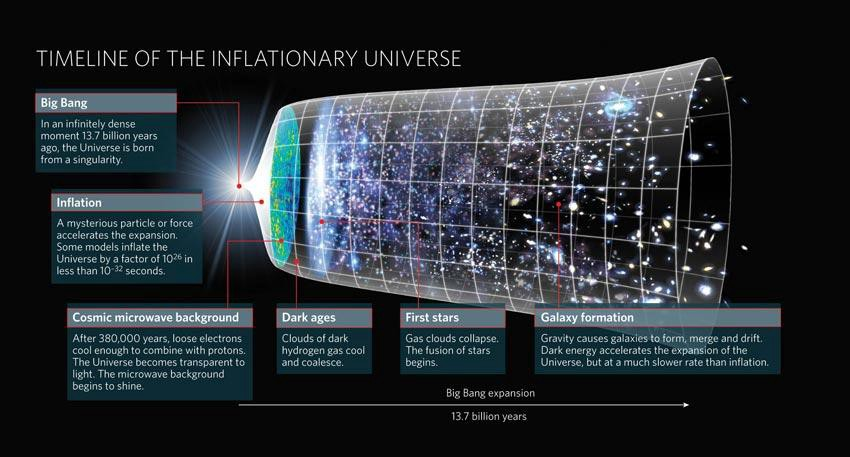
\includegraphics[width=\textwidth]{figure 9.jpeg}
    \caption{A summary of the evolution of the universe}
    \label{fig:final}
\end{figure}

\newpage

\section{References}
\begin{itemize}
    \item An Introduction to Modern Cosmology 
    , Third Edition by Andrew Liddle
    \item An Introduction to Modern Astrophysics, Second Edition, by Bradley W. Carroll and Dale A. Ostlie.
\end{itemize}


\end{document}
